\chapter{Methodology}
Typical procedure in doing deep neural MD simulation is as follows:

\begin{itemize}
    \item \emph{Data Exploration}. Before training a model, one needs to supply
          first inputs such as	atom type, the simulation box, atom
          coordinates, etc.	 Initial trajectories were generated
          using Molecular Dynamics implemented in
          LAMMPS \cite{LAMMPS}. The pair potential used is based on the
          previously
          trained deep neural network potential (NNP) generated by
          Sanchez-Burgos et
          al.
          \cite{sanchez2023deep}.

          For the MD simulation, a system size of 192 water molecules was used
          for both
          the bulk and interface systems, as shown in Figure
          \ref{fig:cryst_sctruct}. The
          temperature was varied from 300 K to 600 K. The simulation profile of
          the bulk
          system is as follows: NPT ensemble at 1 bar for 2 ns, and a ramp from
          1 bar to
          10,000 bar for 10 ns. For the interface system, the simulation was
          done in
          NVT
          ensemble for 10 ns and the box size was based on the average length
          of the
          corresponding bulk system at a given temperature and at 1 bar. Vacuum
          was
          introduced as to create a total length of 50 \r{A} in the direction
          normal to
          the interface. For both systems,
          Nosé-Hoover thermostat  with a
          relaxation time of 20 fs, and  Nosé-Hoover barostat with a relaxation
          time of 200 fs were
          applied. The equations of motion were integrated
          using the time-reversible measure-preserving Verlet and rRESPA
          integrators derived by Tuckerman et al. \cite{Tuckerman2006} with a
          simulation step of 0.2 fs.

          \begin{figure}[tbhp]
              \centering
              \begin{subfigure}{0.42\textwidth}
                  \centering
                  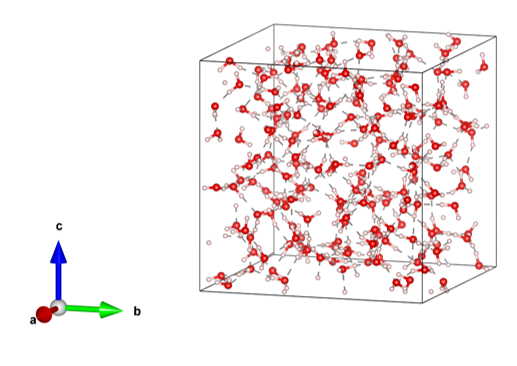
\includegraphics[width=0.75\textwidth]{bulk}
                  \caption{}
                  % \label{fig:}
              \end{subfigure}
              % \hfill
              \begin{subfigure}{0.42\textwidth}
                  \centering
                  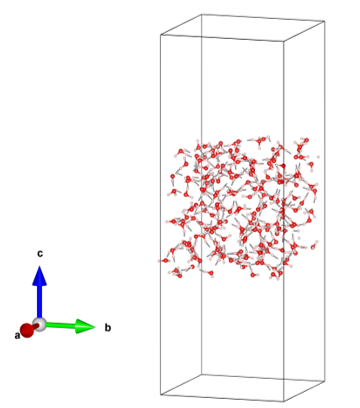
\includegraphics[width=0.75\textwidth]{interface}
                  \caption{}
                  % \label{fig:}
              \end{subfigure}
              \hfill
              \caption{Typical configurations for (a) bulk and (b) interface
                  systems.}
              \label{fig:cryst_sctruct}
          \end{figure}

    \item \emph{Data Labeling}.
          The trajectories were then labeled with their energy, force, and
          pressure
          tensor using Density Functional Theory (DFT) implemented in Quantum
          Espresso
          \cite{QE-2009,QE-2017,QE-2020}. Strongly Constrained and
          Appropriately
          Normed
          (SCAN) exchange-correlation functional is widely used in the study of
          water
          systems due to its great predictability in describing hydrogen bonds
          and
          van
          der Waals interactions \cite{sun2015strongly, chen2017ab}. However,
          for
          this
          study, the SCAN functional tends to be numerically unstable when
          implemented
          to systems with interfaces. Instead, this study tried to use a
          similar but accurate
          and
          numerically efficient r$^2$SCAN meta-generalized gradient
          approximation
          \cite{Furness2020}. Optimized Norm-Conserving Vanderbilt
          pseudopotentials
          \cite{hamann2013optimized} were used with energy cutoff of 130 Ry and
          scf
          convergence threshold of \num{1e-6} Ry.

    \item \emph{Training}. The labeled frames were then feed into DeePMD-kit
          code
          \cite{wang2018deepmd,zeng2023deepmd,lu2021,zhang2018end} for the
          training
          of
          deep neural network potentials. A total of 1200 original bulk frames
          and 1000 original
          interface
          frames were used as training data. The training follows a typical
          two-neutral
          network architecture. First, atomic configurations are processed by
          the
          embedding network of three layers consisting of 25, 50 and 100
          neurons
          each.
          The embedding follows the two-body smooth-edition scheme
          \cite{zhang2018end}
          that conserves radial and angular information within the cutoff
          radius of 6
          \r{A}. A switching function was applied for atoms beyond 5.5 \r{A} to
          ensure
          smooth cutoff.	Then, the atomic descriptors are build and
          given as
          input to a
          fitting network of three layers of 250 neurons each that outputs a
          scalar
          quantity such as energy. The parameters of the neural network are
          set
          during
          the training procedure by minimizing	loss function based on the mean
          squared
          error on the total energy and atomic forces predicted
          by the network with respect to the reference data. The minimization
          started with a large prefactor on the forces and ended with equal
          prefactors
          for both forces and energies.    The iterative
          minimization
          was performed with a total of 3 million batches and a learning rate
          that
          exponentially decay from \num{1e-3} to \num{3.5e-8}. Once the
          training is finished, the trained neural network will be  ``freezed''
          or dumped into a protobuf(.pb) file that can be used as a pair
          potential during MD simulation.

    \item \emph{Testing}. The neural network potential was tested by
          comparing results predicted by the NN potential with	  the results
          of DFT
          calculation on the validation datasets.

    \item \emph{Run MD}. Once the NN model is good, one can perform molecular
          dynamics simulations using the trained neural   network potential to
          predict
          system's properties of interest.

    \item \emph{Check Deviation}. It is possible that during stochastic
          gradient descent runs, the NN model reached a different local minima.
          Hence,
          the common procedure is to train multiple similar models but
          different
          initialization by providing a  random seed. These models will be used
          to run MD simulations and deviations among these models will then be
          compared. Larger deviation for structure properties (default is the
          atomic
          force) means less accuracy of the models. Using this criterion, a few
          trajectories whose max force standard deviation is within a lower and
          higher
          threshold of 0.8 \unit{eV/\angstrom} and 1.5	\unit{eV/\angstrom},
          respectively,
          will be selected and put into the next iteration. Each iteration will
          execute data labeling  and  the new data will be put together with
          initial data
          and data generated in previous iterations for the training. This is
          called active learning. For this work, five iterations were applied
          on
          the bulk
          systems with a total training data of 6080 frames.

    \item \emph{Obtain relevant properties}. Once the MD
          simulation is
          finished, one can compute properties of the system such as density,
          surface
          tension, and dipole orientation.	 The mass density was fitted according to the formula \cite{sanchez2023deep}

          \begin{equation}
              \rho(z) = \frac{\rho_l+\rho_v}{2} -  \frac{\rho_l-\rho_v}{2} \tanh\left(\frac{z-z_0}{d} \right)
              \label{eq:fit_dens}
          \end{equation}

          where  $\rho_l$ and $\rho_v$ are the  coexistence liquid and vapor densities, respectively,  $z_0$ the position of the interface, and $d$ its thickness.


          The surface tension can be
          calculated according to Kirkwood-Buff
          equation
          \cite{kirkwood1949} given by

          \begin{equation}
              \gamma = \frac{L_z}{2} \left[ \expval{P_{zz}} -\frac{1}{2} \left(
                  \expval{P_{xx}} + \expval{P_{yy}} \right) \right]
              \label{eq:surf_tens}
          \end{equation}

          where $\expval{P_{ij}}$ is the $ij$th element of the pressure tensor,
          and $L_z$ is the total length of the box size in the direction normal
          to the
          surface.

\end{itemize}
